% v2-acmsmall-sample.tex, dated March 6 2012
% This is a sample file for ACM small trim journals
%
% Compilation using 'acmsmall.cls' - version 1.3 (March 2012), Aptara Inc.
% (c) 2010 Association for Computing Machinery (ACM)
%
% Questions/Suggestions/Feedback should be addressed to => "acmtexsupport@aptaracorp.com".
% Users can also go through the FAQs available on the journal's submission webpage.
%
% Steps to compile: latex, bibtex, latex latex
%
% For tracking purposes => this is v1.3 - March 2012

\documentclass[prodmode,acmtecs]{acmsmall} % Aptara syntax

\usepackage{subfig}
\usepackage{epsfig}
\usepackage{amsmath,amsfonts,amssymb,amstext}
\usepackage{natbib,multirow}

% Package to generate and customize Algorithm as per ACM style
\usepackage[ruled]{algorithm2e}
\renewcommand{\algorithmcfname}{ALGORITHM}
\SetAlFnt{\small}
\SetAlCapFnt{\small}
\SetAlCapNameFnt{\small}
\SetAlCapHSkip{0pt}
\IncMargin{-\parindent}

% Metadata Information
\acmVolume{0}
\acmNumber{0}
\acmArticle{0}
\acmYear{0}
\acmMonth{0}

% Copyright
%\setcopyright{acmcopyright}
%\setcopyright{acmlicensed}
%\setcopyright{rightsretained}
%\setcopyright{usgov}
%\setcopyright{usgovmixed}
%\setcopyright{cagov}
%\setcopyright{cagovmixed}

% DOI
%\doi{0000001.0000001}

%ISSN
%\issn{1234-56789}

% Document starts
\begin{document}

% Page heads
\markboth{E. Irurozki et al.}{Algorithm xxx: \texttt{perm\_mateda}: A matlab toolbox of EDAs for permutation-based problems}

% Title portion
\title{Algorithm xxx: \texttt{perm\_mateda}: A matlab toolbox of estimation of distribution algorithms for permutation-based combinatorial optimization problems}
\author{EKHINE IRUROZKI
\affil{Intelligent Systems Group, Basque Center for Applied Mathematics (BCAM)}
JOSU CEBERIO
\affil{Intelligent Systems Group, Faculty of Computer Science, University of the Basque Country UPV/EHU}
JOSEAN SANTAMARIA
\affil{Intelligent Systems Group, Faculty of Computer Science, University of the Basque Country UPV/EHU}
ROBERTO SANTANA
\affil{Intelligent Systems Group, Faculty of Computer Science, University of the Basque Country UPV/EHU}
ALEXANDER MENDIBURU
\affil{Intelligent Systems Group, Faculty of Computer Science, University of the Basque Country UPV/EHU}}




% NOTE! Affiliations placed here should be for the institution where the
%       BULK of the research was done. If the author has gone to a new
%       institution, before publication, the (above) affiliation should NOT be changed.
%       The authors 'current' address may be given in the "Author's addresses:" block (below).
%       So for example, Mr. Abdelzaher, the bulk of the research was done at UIUC, and he is
%       currently affiliated with NASA.

\begin{abstract}
Permutation problems are combinatorial optimization problems whose solutions are naturally codified as permutations. Due to their complexity, motivated principally by the factorial cardinality of the search space of solutions, they have been a recurrent topic for the artificial intelligence and operations research community. Recently, among the vast number of metaheuristic algorithms, new advances on estimation of distribution algorithms (EDAs) have shown outstanding performance when solving some permutation problems. These novel EDAs implement distance-based exponential probability models such as the Mallows and Generalized Mallows models. In this paper, we present a Matlab package, \texttt{perm\_mateda}, of estimation of distribution algorithms on permutation problems, which has been implemented as an extension to the Mateda-2.0 toolbox of EDAs.  Particularly, we provide implementations of the Mallows and Generalized Mallows EDAs under the Kendall's-$\tau$, Cayley, and Ulam distances. In addition, four classical permutation problems have been also implemented: Traveling Salesman Problem, Permutation Flowshop Scheduling Problem, Linear Ordering Problem, and Quadratic Assignment Problem.
\end{abstract}

%
% The code below should be generated by the tool at
% http://dl.acm.org/ccs.cfm
% Please copy and paste the code instead of the example below. 
%


\begin{CCSXML}
<ccs2012>
<concept>
<concept_id>10002950.10003624.10003625.10003627</concept_id>
<concept_desc>Mathematics of computing~Permutations and combinations</concept_desc>
<concept_significance>500</concept_significance>
</concept>
<concept>
<concept_id>10002950.10003624.10003625.10003630</concept_id>
<concept_desc>Mathematics of computing~Combinatorial optimization</concept_desc>
<concept_significance>500</concept_significance>
</concept>
</ccs2012>
\end{CCSXML}

\ccsdesc[500]{Mathematics of computing~Permutations and combinations}
\ccsdesc[500]{Mathematics of computing~Combinatorial optimization}


\begin{CCSXML}
<ccs2012>
<concept>
<concept_id>10002950.10003648</concept_id>
<concept_desc>Mathematics of computing~Probability and statistics</concept_desc>
<concept_significance>500</concept_significance>
</concept>
<concept>
<concept_id>10010405.10010481</concept_id>
<concept_desc>Applied computing~Operations research</concept_desc>
<concept_significance>500</concept_significance>
</concept>
</ccs2012>
\end{CCSXML}

\ccsdesc[500]{Mathematics of computing~Probability and statistics}
\ccsdesc[500]{Applied computing~Operations research}

%
% End generated code
%

% We no longer use \terms command
%\terms{Design, Algorithms, Performance}

\keywords{estimation of distribution algorithms, Mallows and Generalized Mallows models,  optimization, permutation-based problems, Matlab}

\acmformat{Ekhine Irurozki, Josu Ceberio, Josean Santamaria, Roberto Santana, Alexander Mendiburu, 2017. \texttt{perm\_mateda}: A matlab toolbox of estimation of distribution algorithms for permutation-based combinatorial optimization problems.}
% At a minimum you need to supply the author names, year and a title.
% IMPORTANT:
% Full first names whenever they are known, surname last, followed by a period.
% In the case of two authors, 'and' is placed between them.
% In the case of three or more authors, the serial comma is used, that is, all author names
% except the last one but including the penultimate author's name are followed by a comma,
% and then 'and' is placed before the final author's name.
% If only first and middle initials are known, then each initial
% is followed by a period and they are separated by a space.
% The remaining information (journal title, volume, article number, date, etc.) is 'auto-generated'.

\begin{bottomstuff}
This work has been partially supported by the Research Groups 2013-2018 (IT-609-13) and BERC 2014-2017 programs (Basque Government), and  TIN2016-78365-R and Severo Ochoa excellence accreditation SEV-2013-0323 programs (Spanish Ministry of Economy and Competitiveness).

Author's addresses: E. Irurozki, Basque Center for Applied Mathematics (BCAM), Alameda de Mazarredo 14, 48009 Bilbao, Bizkaia, Spain; J. Ceberio, J. Santamaria and R. Santana, Computer Science and Artificial Intelligence Department, Faculty of Computer Science, UPV/EHU, 20018 Paseo M. Lardizabal 1, Donostia - San Sebastian, Gipuzkoa, Spain; A. Mendiburu, Computer Architecture and Technology, Faculty of Computer Science, UPV/EHU, 20018 Paseo M. Lardizabal 1, Donostia - San Sebastian, Gipuzkoa, Spain.
\end{bottomstuff}

\maketitle

\section{Introduction}

In combinatorics, many optimisation problems are defined as "the way of ordering $n$ number of items" such that a specific function is maximized (or minimized). Referred to as  {\it permutation-based problems}, or simply {\it permutation problems}, these combinatorial problems are characterized by the fact that their solutions are naturally codified as permutations. Motivated principally by their versatility - ordered sets of items, collection of disjoint cycles, transpositions, matrices or graphs- permutations appear in a vast range of domains, such as graph theory, mathematical psychology or bioinformatics, and, particularly, in logistic problems such as routing~\cite{toth2001}, scheduling~\cite{Gupta2006} or assignment~\cite{Burkard98}. The DNA fragment assembly~\cite{Parsons1995}, vehicle routing~\cite{toth2001} or aircraft landing scheduling~\cite{Beasley2000} problems are examples of the presence of permutation problems in a wide range of real-wold scenarios.

If no constraints are assumed, the search space of solutions is defined as the set of all the permutations of $n$ items ($n!$ solutions in total). Due to the factorial cardinality of the search space, permutation problems are known as very hard problems when $n$ goes above a relatively small number. Indeed, the work of Garey and Johnson~\cite{garey1979} on computational complexity demonstrated that many of these problems are {\it NP-hard}.

In view of their complexity, computing {\it optimal} solutions is intractable in general. For this reason, we are usually satisfied with {\it good} solutions. In this sense, the artificial intelligence community has proposed a large number of metaheuristic algorithms that provide {\it acceptable} solutions in reasonable computation times. Generally, these algorithms neither guarantee the optimality of solutions nor define how close the obtained solutions are from the optimal ones. Among the vast amount of metaheuristic algorithms, tabu search, scatter search, local search, variable neighbourhood search, ant colony optimisation, simulated annealing and genetic algorithms are some of the metaheuristics that have been applied on permutation problems. 

Estimation of Distribution Algorithms (EDAs)~\citep{larranaga2002a,Lozano2005,pelikan2002} have also been applied successfully to permutation problems~\cite{ceberio2014d}. EDAs are population based optimization algorithms that, at each generation, estimate a probability distribution from the set of selected solutions in order to represent the (in)dependencies between the variables. Then, the new solutions are obtained by sampling the probability distribution estimated in the previous step. This process (hopefully) leads the algorithm towards the optimal solutions. Different EDAs have been proposed for discrete, continuous and mixed problems. Many works in the literature confirm the good performance of EDAs in artificial as well as real-world problems: Protein Folding~\citep{armananzas2008}, Capacitated Vehicle Routing Problems~\citep{tsutsui2004}, Calibration of Chemical Applications~\citep{Mendiburu2006}, Finding the Optimal Path in 3D Spaces~\citep{Yuan2007}, Software Testing~\citep{Sagarna2006}, Chemotherapy Treatment Optimization for Cancer~\citep{Brownlee2008}, Nuclear Reactor Fuel Management Parameter Optimization~\citep{Jiang2006}, Dynamic Pricing~\citep{McCall2012} or Molecular Docking~\citep{Soto2012}.

A recent review by~\citet{ceberio2011b} studied the performance of several classical EDAs, confirming that, in general, when applied to permutation-based problems, they are not very competitive. The permutation codification of solutions represents a real challenge for EDAs, since classical probability distributions on the discrete or continuous domains can not be efficiently adapted to deal with permutation solutions. Notions, such as variable independence, are not naturally translated into the domain of permutations since, in contrast to integer problems, two given positions in a permutation can not ever have the same value. This simple constraint, known as the {\it mutual exclusivity constraint}~\citep{huang2009}, requires in general a more complex mathematical machinery in order to deal efficiently with the permutation nature of the solutions.

In order to overcome this drawback, several distance-based probability models, such as the Mallows and the Generalized Mallows models have been included in the context of EDAs~\citep{ceberio2011a,ceberio2011c,ceberio2013a,ceberio2013b,ceberio2014c}. This step opens new research lines, both methodological and applied, in a topic (solving permutation problems) of growing interest in the literature. In fact, Mallows and Generalized Mallows models have been recently addressed in a number of papers~\cite{ALEDO2017299,ALEDO2016308,ZANGARI2017137}, and EDAs based on these models have been successfully applied in real world problems such as permutation flowshop scheduling~\cite{ceberio2013a}, aircraft arrival sequencing~\cite{Ji2016,Ji2016a}, network design~\cite{Anton-Sanchez2017} and routing problems~\cite{PEREZRODRIGUEZ2017288}.

Taking into account its potential, and with the aim of providing a powerful tool for the community, we present a complete framework of EDAs for permutation problems in Matlab, which is implemented as an extension to the Mateda-2.0 toolbox of EDAs developed by~\citet{Santana2010}. Particularly, we focus on two distance-based exponential probability models, called the Mallows model~ \cite{mallows1957} and the Generalized Mallows model~\cite{fligner1986}. In order to enhance the applicability and robustness of this framework, based on these two models, we present five different EDAs  (combinations of two models with the distance-metrics): the Mallows EDA (MEDA) and the Generalized Mallows EDA (GMEDA), under the Kendall's-$\tau$, Cayley and Ulam distance-metrics\footnote{Due to theoretical restrictions, the Generalized Mallows model under the Ulam distance has not been considered.}.  In addition, four classical permutation problems have been also implemented: Traveling Salesman Problem (TSP)~\cite{goldberg1985}, Permutation Flowshop Scheduling Problem (PFSP)~\cite{Gupta2006}, Linear Ordering Problem (LOP)~\cite{ceberio2014a}, and Quadratic Assignment Problem (QAP)~\cite{koopmans1955}.

Complementary to this manuscript, a user's manual with installation, implementation and usage details of \texttt{perm\_mateda} toolbox is provided. Any practitioner interested in the implementation of EDAs for solving permutation problems is referred to address the user's manual.

The remainder of the paper is structured as follows: in the next section, a brief introduction on EDAs is given. In Section~\ref{sec:GM}, the Mallows and Generalized Mallows models under the  Kendall's-$\tau$, Cayley and Ulam distances are introduced. Section~\ref{sec:permproblems} describes the four permutation problems implemented in the toolbox. Afterwards, Section \ref{sec:experiments} presents some experimental runs of EDAs implemented in \texttt{perm\_mateda} and tested on instances of three permutation problems. Finally, conclusions and ideas for future work are presented in Section~\ref{sec:conclusions}.

\section{A brief review of EDAs on Mateda-2.0}\label{sec:EDAs}

Algorithm~\ref{alg:EDA} provides the general overview of EDAs. The methods the user can implement or adapt are highlighted in italics.

\begin{algorithm}[t]
\SetAlgoNoLine
$t=0$\;
Generate  an initial population $D_t$ using a \emph{seeding method}\;
If required, apply a \emph{repairing method} to $D_t$\;
Evaluate (all the objectives of) population $D_t$ using an \emph{evaluation method}\;
If required, apply a \emph{local optimization method} to $D_t$\;
\While{The termination criterion is not met}{
Select a set $D_t^S$ of points from $D_t$ according to a \emph{selection method}\;
Compute a probabilistic model of $D_t^S$ using a \emph{learning method}\;
Sample a $D_{Sampled}$ population using a \emph{sampling method}\;
If required, apply a \emph{repairing method} to $D_{Sampled}$\;
Evaluate (all the objectives of) population $D_{Sampled}$ using an \emph{evaluation method}\;
If required, apply a \emph{local optimization method} to $D_{Sampled}$\;
$t = t+1$\;
Create $D_t$ population from populations $D_{t-1}$ and $D_{Sampled}$  using a \emph{replacement method}\;
}

\caption{General pseudocode of Estimation of Distribution Algorithms (EDAs)}\label{alg:EDA}
\end{algorithm}

EDAs begin with the generation of an initial set of solutions (usually called a population). Although the first population is usually randomly generated, it can be done using a particular heuristic or \emph{seeding method} in some situations, e.g., when previous information about the approximate location of the optimal solutions is available.

\emph{Selection methods} serve to identify the subset of solutions that will be used to learn the probabilistic model. This subset usually gathers the solutions with the best value, according to the evaluation function defined for the optimization problem at hand. 

The \emph{learning method} is a characteristic and critical component of EDAs. Depending on the class of probability models used, this step involves parametric or structural learning, also known as model fitting and model selection, respectively.

\emph{Sampling methods} are used to generate new solutions from the learned probabilistic model. They depend on the type of probabilistic model and the characteristics of the problem. In addition, they can be conceived to deal with certain types of constraints in the solutions.

\emph{Repairing methods} should be applied for constrained problems where  sampled solutions may be infeasible and some strategy to repair these solutions is available.

The \emph{evaluation method} comprises the call to the evaluation function (which measures the quality of the solutions). For multi-objective problems this may imply the evaluation of a set of functions. An advantage of EDAs and other evolutionary algorithms is that the evaluation function does not have to be differentiable or even continuous.

EDAs are global optimization algorithms and their results can be improved when used together with \emph{local optimization methods} that perform some local search departing from the current solution.

\emph{Replacement methods} combine the solutions stored in the previous generation with the current set of sampled solutions. These methods can help to retain the best solutions found so far, maintain the diversity in the population, etc.

Finally, the \emph{termination criteria method} determines the stopping conditions for the EDA algorithm. These criteria can be as simple as a fixed number of generations or may imply a statistical analysis of the current population.

Mateda-2.0 provides a suitable modular framework to implement EDAs for permutation problems. The design of the new algorithms can be mainly focused on the implementation of new \emph{learning} and \emph{sampling methods}. In addition, for real-world permutation problems other modules could be also modified, such as \emph{local optimization} or \emph{selection methods}.


\section{The Mallows and Generalized Mallows models}~\label{sec:GM}

Before going into the details on probability models, some notation on permutations and distances is required. 
Throughout this section, permutations will be in general denoted as $\sigma$ or $\pi$. By $\pi^{-1}$ the inverse permutation of $\pi$ is denoted. The composition of $\sigma$ and $\pi$ is stated as $\sigma \pi$, and implies $\sigma\pi(i)=(\sigma\circ\pi(i))=\sigma(\pi(i))$. The permutation $e$ stands for the identity permutation, i.e., $e=1234 \ldots n$. Distance $d(\sigma, \pi)$ measures the disagreements between the two permutations and, for convenience, $d(\sigma, e)$ is denoted as $d(\sigma)$. For every distance considered in this manuscript, the right invariance property holds, i.e., $d(\sigma, \pi)=d(\sigma\pi^{-1}, e)=d(\sigma\pi^{-1})$.

The Mallows model \cite{mallows1957} is a distance-based exponential probability model over permutation spaces.  Given a distance over permutations, the Mallows model is defined by two parameters: the central permutation $\sigma_0$, and the spread parameter $\theta$. Formally, the probability of every permutation $\sigma$ under the Mallows model is defined as follows:
\begin{equation}
P(\sigma) =\psi(\theta)^{-1} \exp(-\theta d(\sigma, \sigma_0))  	
\label{eq:mallows}
\end{equation}
where $\psi(\theta)$ denotes the normalization constant, and $d(\sigma,\sigma_0)$ denotes the distance between $\sigma$ and $\sigma_0$ for a distance metric among permutations. When $\theta>0$, $\sigma_0$ is the permutation with the highest probability value (the mode), and the probability of the other $n!-1$ permutations decreases exponentially with the distance to the central permutation. Roughly speaking, the closer a permutation $\sigma$ to $\sigma_0$, the higher its probability. Moreover, when $\theta=0$, we obtain the uniform distribution and, as $\theta$ increases, the distribution becomes more concentrated around the central permutation $\sigma_0$.

As an extension to the Mallows model, the Generalized Mallows (GM) model was proposed in~\cite{fligner1986}. Like the Mallows model, the GM is exponential and unimodal. However, instead of using a single spread parameter $\theta$, the GM model makes use of a $(n-1)$-dimensional spread parameter $\boldsymbol{\theta}=(\theta_1, \theta_2, ... \, , \theta_{n-1})$, where each $\theta_j$ affects a particular position in the permutation, and $n$ is the size of the permutation. This allows modeling a distribution with more emphasis on the consensus of certain positions of the permutation while having more uncertainty in others. 

Before going into details, it is worth stating that not every distance that can be considered for the Mallows model can also be implemented for the GM model (this is the case of the Ulam distance-metric). In fact, the GM model requires the distance-metric to be decomposed as the sum of $n-1$ terms. 
\begin{equation}
d(\sigma, \sigma_0)=\sum_{j=1}^{n-1}S_j(\sigma\sigma_0^{-1})
\label{eq:decomp}
\end{equation}

The vector grouping the terms $\mathbf S(\sigma\sigma_0^{-1}) = ( S_1(\sigma\sigma_0^{-1}), \ldots , S_{n-1}(\sigma\sigma_0^{-1}) )$ is denoted as the distance decomposition vector. The GM model, whose definition relies on this vector, is expressed as:

\begin{equation}
P(\sigma)= \psi(\boldsymbol{ \theta})^{-1} \exp\left( \sum_{j=1}^{n-1}-\theta_j S_j(\sigma \sigma_0^{-1})\right)
\label{eq:gmallows}
\end{equation}

In what follows, we introduce in detail the Kendall's-$\tau$, Cayley and Ulam distances, together with the methods defined to learn and sample the Mallows and GM models under each of these distance-metrics. Further discussion about Mallows and GM models with the three distances, as well as several different sampling and learning algorithms, can be found in ~\cite{irurozki2014d} and~\cite{irurozki2014c}. 


It is worth to mention that, according to~\cite{ceberio2014c}, there is no one best distance-metric in general. Interestingly, some distances behave good for some problems (meaning that it will perform good for most instances of the problem) and other distances for other problems.
Despite not being possible to make an exhaustive correspondence between distances and problems, as a general rule we can state that an EDA under a particular distance-metric will perform good for a problem in a certain domain if that metric is adequate to measure the discrepancies of the permutations in that domain. In the following sections, we present the distance-metrics on permutations considered in the toolbox, and emphasize the type of discrepancies they measure. Later, in the experimental section, we will propose a possible correspondence between these metrics and the considered permutation problems.

In the following section we do not include any Matlab code. It is provided together with additional explanations in the user manual.

\subsection{Kendall's-$\tau$ distance}
The Kendall's-$\tau$ distance $d_\tau(\sigma , \pi)$ counts the number of pairwise disagreements between $\sigma$ and $\pi$.
\begin{align*}
d_\tau(\sigma, \pi)=|\{(i,j) : i<j,\,\, & (\sigma(i) < \sigma(j) \land \pi(i)>\pi(j) ) \\
 \lor & (\pi(i) < \pi(j) \land \sigma(i)>\sigma(j) )  \, \}|
\end{align*}
It is the best choice when our permutations are interpreted as rankings (in recommender systems for example). It is equivalent to counting the number of adjacent swaps to convert $\sigma^{-1}$ into $\pi^{-1}$. The Kendall's-$\tau$ distance $d_\tau(\sigma)$ can be broken down into a distance decomposition vector $\mathbf V(\sigma)=(V_1(\sigma), \ldots, V_{n-1}(\sigma))$, which is also referred to as \textit{inversion vector}, and can be expressed as follows: 


\begin{equation}
 V_j(\sigma) = \sum_{i=j+1}^n \bm{1}_{[\sigma(i) < \sigma(j)]}
 \label{eq:kendall_decomp}
\end{equation}
It follows that $V_j(\sigma)$ is equal to the number of items of higher index than $j$ that are smaller than $\sigma(j)$ and it ranges for $0\leq V_j(\sigma) \leq n-j$ for $1\leq j \leq n$. As an example, if $\sigma=2 1 3 6 4 5$, then $V(\sigma)=(1 0 0 2 0)$ and $d_\tau(\sigma)=\sum_{j=1}^{n-1} V_j(\sigma)=3$.  The conversion from $\mathbf V(\sigma)$ to $\sigma$ and vice versa is carried out in $O(n^2)$. 

The spread parameter $\boldsymbol\theta$ of the GM model under the Kendall's-$\tau$ distance is an $(n-1)$-dimensional vector. Let $\sigma$ be a permutation sampled from a GM model under the Kendall's-$\tau$ distance, with parameters $\boldsymbol\theta$ and $\sigma_0$, where $\sigma_0(j)=i$. The spread parameter $\theta_j$ is related to position $j$ in $\sigma$ in the sense that, the larger $\theta_j$, the larger the probability of $\sigma(j)\leq i$. When permutations are interpreted as rankings, this means that item $j$ is ranked in the first $i$ positions with high probability. Further details of the Mallows and GM models under this distance can be found in~\cite{fligner1986}.


\subsection{Cayley distance}
The Cayley distance $d_c(\sigma, \pi)$ counts the minimum number of swaps (not necessarily adjacent) to transform $\sigma$ into $\pi$. The Cayley distance is related to the concept of cycles in $\sigma$, defined as ordered sets $\{i_1, \ldots , i_s\} \subseteq \{1, \ldots , n\}$ such that $\sigma(i_1) = i_2$, $\sigma(i_2) = i_3$, \ldots , $\sigma(i_s) = i_1$. When the reference permutation is the identity, $d_c(\sigma)$ equals $n$ minus the number of cycles in $\sigma$. 


The distance decomposition vector $\mathbf X(\sigma)= (X_1(\sigma), \ldots, X_{n-1}(\sigma))$ of the Cayley distance has length $n-1$ and each term can be expressed as follows:

\begin{equation}
X_j(\sigma) =
 \begin{cases}
   0 & \text{iff  $j$ is the largest item in its cycle in $\sigma$,} \\
   1       & \text{otherwise. }
  \end{cases}
 \label{eq:cayley_decomp}
\end{equation}

Given $\sigma=2 1 3 6 4 5$, its corresponding cycle notation is $(2 1)(3)(4 5 6)$, the distance decomposition vector is $X(\sigma)=1 0 0 1 1$ and $d_c(\sigma)=\sum_{j=1}^{n-1} X_j(\sigma)=3$. This conversion from $\sigma$ to $\mathbf X(\sigma)$ can be run in $O(n)$.% In this case, as done for Kendall's-$\tau$, two methods are also defined in Table~\ref{T:SamplingMethods}: xVector (to obtain the corresponding decomposition) and GeneratePermuFromX (to obtain a permutation associated to a given $X$ decomposition). 

Like the GM model under the Kendall's-$\tau$, the GM model (Eq.~\ref{eq:gmallows}) under the Cayley distance considers an $(n-1)$-dimensional vector spread parameter $\boldsymbol\theta$. So, again, the larger $\theta_j$, the larger the probability that $\sigma(j)\leq i$. For further discussion on the Cayley distance, we refer the interested reader  to~\cite{Irurozki2016}.

\subsection{Ulam distance}
The Ulam distance $d_u(\sigma,\pi)$ counts the length of the complement of the longest common subsequence (LCS) in $\sigma$ and $\pi$, i.e., the number of items which are not part of the LCS. If the reference permutation is the identity, $d_u(\sigma)$ equals $n$ minus the length of the longest increasing subsequence (LIS). 

The classical example to illustrate the Ulam distance, $d_u(\sigma, \pi)$, considers a shelf of books in the order specified by $\sigma$ \citep{diaconis1988}. The objective is to order the books as specified by $\pi$ with the minimum possible number of movements, where a movement consists of taking a book and inserting it into another position (delete-insert). The minimum number of movements is exactly $d_u(\sigma, \pi)$. 

For example, given $\sigma=2 1 3 6 4 57$, the length of the LIS\footnote{Note that there can be more than one sequence with the same LIS value. In this case, there are two sequences: 13457 and 23457.} is 5 and, therefore, $d_u(\sigma)=2$. 

The computation of the Ulam distance between two given permutations has complexity $O(n \, log \, l)$ where $l$ is the length of the longest common subsequence. 

Currently, no distance decomposition vector for the Ulam distance has been reported in the literature. Consequently, the GM model can not be extended to the Ulam distance. More details in this regard can be found in~\cite{irurozki2014e}.

\subsection{Learning \& Sampling}
Learning the parameters of the Mallows or GM models given a sample of permutations is either known or conjectured to be NP-Hard for all the distance-metrics considered in this manuscript. Note that there exist several approaches to learn the models considered in this paper~\cite{irurozki2014d}. In this sense, EDAs do not require the model that most accurately represents the selected solutions to be learned in each generation. This is so because approximate models can be beneficial to explore other areas of the search space. Moreover, approximate algorithms are computationally more affordable than exact approaches, which is also desirable. Therefore, the learning step is usually split into two stages as follows: 
\begin{enumerate}
 \item Approximate the central permutation $\sigma_0$. 
 \item Obtain the maximum-likelihood estimator (MLE) of the spread parameter(s), $\boldsymbol\theta$, for the given distance. 
\end{enumerate}

For step (1), we considered three different alternatives, which are:
\begin{itemize}
\item {\it Borda}~\cite{borda1781}: Selects as the central permutation the result of sorting the items in descending order according to their average position across all the input permutations. When the permutations come from a Mallows model under the Kendall's-$\tau$ distance, the Borda permutation is an asymptotically optimal estimator of the central permutation \cite{Fligner1988}. Note that, although it can be used for any type of distance-metric, we recommend to consider it exclusively for the Kendall's-$\tau$ distance.
\item {\it SetMedianPermutation}: Selects the individual in the sample that minimizes the sums of distances to the rest (given a particular distance).  
\item {\it BestPermutation}: Chooses the permutation with the best evaluation (objective) value.
\end{itemize}

In step (2), once the central permutation $\sigma_0$ has been obtained, the spread parameter(s) are estimated. In the case of MLE, the expression for these parameter(s) is obtained by equating the derivative of the likelihood to zero. Although these expressions differ for each distance, in most of the cases numerical methods can be used to obtain an approximate value. Exact expressions can be found in \cite{irurozki2014c,irurozki2014e,irurozki2014d,Mandhani2009}.

The sampling process consists of generating a representative sample from a distribution, which in our case means generating permutations from the model obtained in the learning stage. The sampling algorithm depends on the distance considered in the model. 

Mallows and GM models under the Kendall's-$\tau$ and Cayley distances can be factorized, leading to efficient sampling algorithms. Roughly speaking, given the distributions obtained in the previous learning step, the sampling step, first, randomly generates decomposition vectors, and then converts the vector to a permutation. Clearly, the complexity of the sampling process depends on the complexity of each of these two steps.
Details of the sampling algorithms for both distances can be found in \cite{irurozki2014d} called Multistage sampler. 

In the case of Ulam, randomly generating permutations is equivalent to randomly generating Young Tableaux, combinatorial objects from representation theory. Details can be found in \cite{irurozki2014d} by the name of Distances sampler.

\section{Permutation problems}\label{sec:permproblems}

Mateda-2.0 toolbox includes implementations of discrete and continuous optimization problems. Following the same idea, we have incorporated four problems defined on permutations: Traveling Salesman Problem (TSP), Permutation Flowshop Scheduling Problem (PFSP), Linear Ordering Problem (LOP), and Quadratic Assignment Problem (QAP). These problems are challenging and they appear frequently in the literature.

Each problem is defined by two modules: one for reading the instance file and processing the parameters (\texttt{Read\{TSP,PFSP,LOP,QAP\}Instance}), and the other for evaluating the solutions (permutations)  (\texttt{Eval\{TSP,PFSP,LOP,QAP\}}).

Although the problems described above have similar methods to read and evaluate, each of them has its own structure and, thus, the data stored for each problem is different: 

\begin{itemize}
\item Traveling Salesman Problem (TSP): This problem is described by one matrix of size $n \times n$ containing the distances between the cities. The TSP implementation can work with both symmetric and asymmetric matrices. Once the data is read, the distance matrix of the problem and the number of cities are stored, in this order, in a global variable named \textit{TSPInstance}.
\item Permutation Flowshop Scheduling Problem (PFSP): The data is contained in one matrix of size $m \times n$ containing the processing times for executing job $j$ for $j={1,2,\ldots,n}$ in machine $i$ for $i={1,2,\ldots,m}$. The matrix that contains the processing times, the number of machines, and the number of jobs are stored, in this order, in a global variable named \textit{PFSPInstance}.
\item Quadratic Assignment Problem (QAP): The data is contained in two matrices of size $n \times n$. The first matrix contains the flow between the facilities and the second one the distances between the locations. Once the data is read,  the distance matrix, flow matrix and problem size are stored, in this order, in a global variable named \textit{QAPInstance}.
\item Linear Ordering Problem (LOP): It is described by one matrix of size $n \times n$ with arbitrary natural numbers. Once the data is read, the matrix and  problem size are stored, in this order, in a global variable named \textit{LOPInstance}.
\end{itemize}

\section{Experimental Study}\label{sec:experiments}
In this section, in order to show the usefulness of the proposed toolbox, we carry out an experimental run of three EDAs on three permutation problems. Specifically, we chose one instance of PFSP, QAP and LOP, {\it tai50\_20\_0}, {\it tai40b} and {\it N-be75eec} respectively, downloaded from well known on-line benchmarks (Taillard's benchmark, QAPLIB and LOLIB). For each problem, one algorithm  implemented in \texttt{perm\_mateda} has been selected (following the comments in~\cite{ceberio2014c} and considering the suitability of each distance-metric for the enumerated problems): for the PFSP, the Generalized Mallows EDA under the Kendall's-$\tau$ distance, for the QAP, the Generalized Mallows EDA under the Cayley distance, and for the LOP the Mallows EDA under the Ulam distance. The code implemented to carry out this experimental study is provided as an example in the User's Manual.

\subsection{Settings}
The parameters setting for in the experimentation is:
\begin{itemize}
\item Population size: $10n$
\item Selection method: the best $10\%$ solutions are selected by truncation.
\item Replacement method: population aggregation. The population is updated by adding the newly created $10n$ solutions and preserving $10n$ solutions with the best evaluation value.
\item Stopping criterion: 500 generations.
\item The learning algorithm is \textit{SetMedianPermutation} in all cases.

\end{itemize}

Each $algorithm-instance$ pair has been run 50 times, and the results have been summarized as the average error with respect to the best known solutions reported in the literature. The exact details of the results can be found in Table~\ref{tab:results}.
\begin{table}
\centering 
\caption{Summary of the results obtained by the three algorithms across the 50 repetitions on the three problems (instances) considered in the experimental study.}
\begin{tabular}{ll|r|rrr}
Problem & Instance & Algorithm & Best Known & Avg. Result & Avg. Time\\\hline
PFSP & tai50\_20\_0 & GMEDA$_K$ & 125831 & 129650.64 & - \\
QAP & tai40b & GMEDA$_C$ & 637250948&  874527286.46 & - \\
LOP &N-be75eec & MEDA$_U$ & 236464 & 213961.78 &  -\\
\end{tabular}
\label{tab:results}
\end{table}

In addition, from the log information stored by the toolbox during the optimization process, it is possible to illustrate the behavior of the algorithm when solving a particular instance. Fig~\ref{fig:convergence_fitness} shows the best evaluation value of the individuals in the population across $500$ generations. It is worth to remark that the purpose of this experimentation is not to provide state-of-the-art results, but to show the flexibility and power of this new toolbox.
\begin{figure}[!hbt]
\begin{center}
\subfloat[GMEDA - Kendall\newline tai50\_20\_0 (PFSP).]{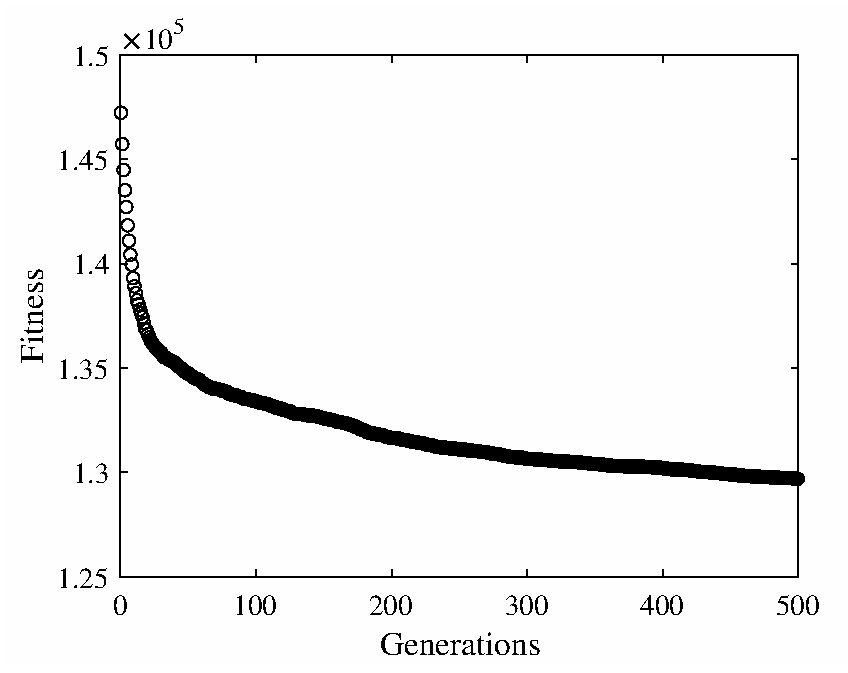
\includegraphics[width=4.0cm]
{Figures/TOMs_Problem_WithBest_3_Fitness.eps}}
\subfloat[GMEDA - Cayley\newline tai40b (QAP).]{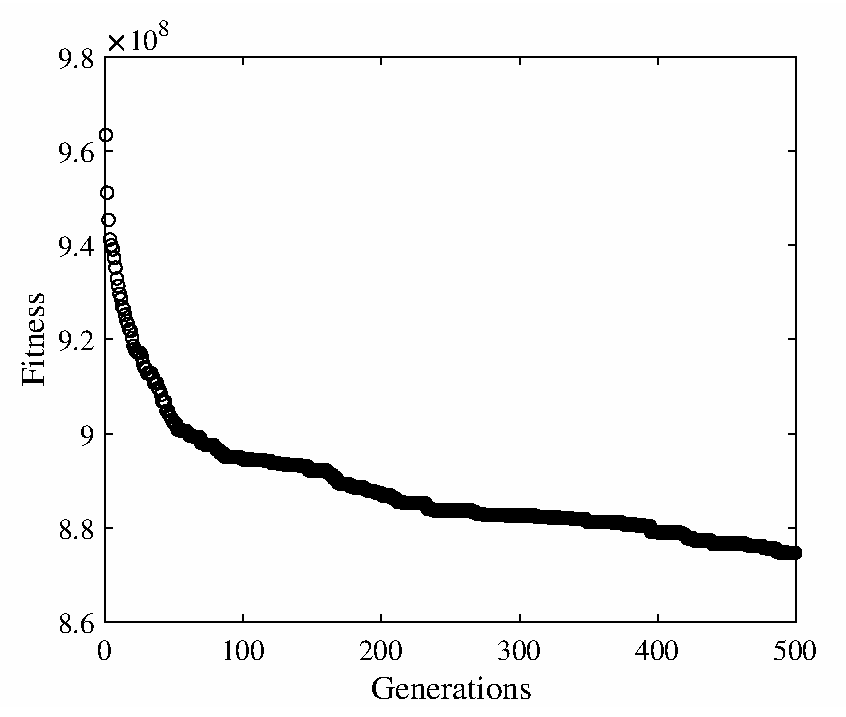
\includegraphics[width=4.0cm]{Figures/TOMs_Problem_WithBest_2_Fitness.eps}} \hspace{0.5cm}
\subfloat[MEDA - Ulam\newline N-be75eec (LOP).]{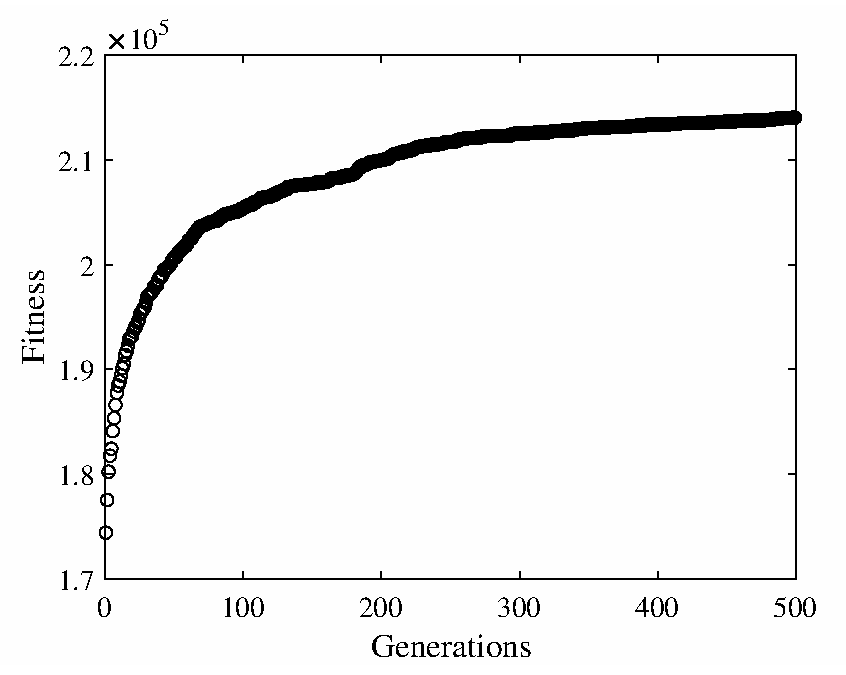
\includegraphics[width=4.0cm]
{Figures/TOMs_Problem_WithBest_1_Fitness.eps}} \hspace{0.5cm}
\end{center}
\caption[caption]{Convergence plots of the population average fitness values obtained through out the optimization (averaged across 50 repetitions).}
\label{fig:convergence_fitness}
\end{figure}

Additionally, using the information stored about the probabilistic model, in Fig~\ref{fig:thetas} the evolution (convergence) of the $\theta$ variable has been illustrated. In the GMEDA cases, in each generation, the average of the $n-1$ parameters have been displayed.
\begin{figure}[!hbt]
\begin{center}
\subfloat[GMEDA - Kendall\newline tai50\_20\_0 (PFSP).]{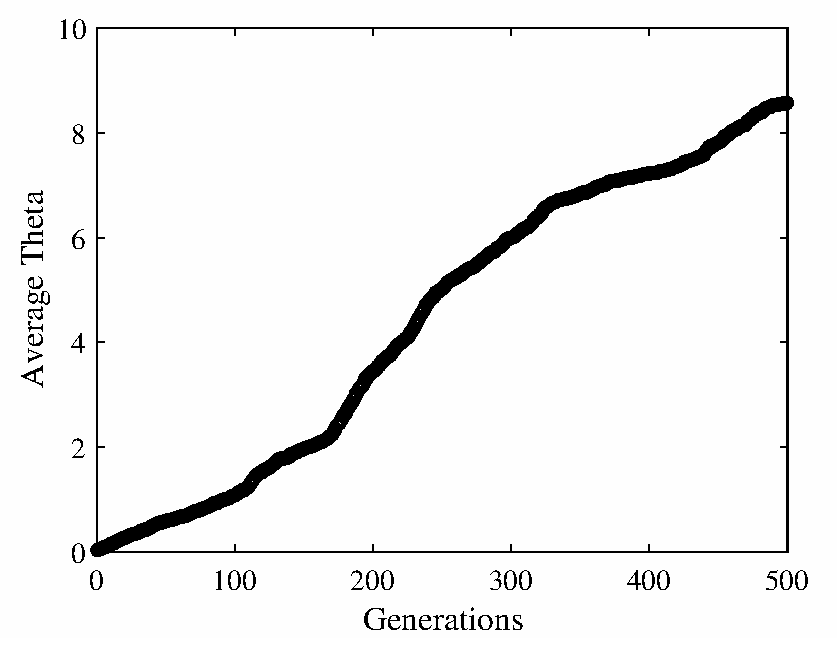
\includegraphics[width=4.0cm]
{Figures/TOMs_Problem_WithBest_3_Theta.eps}}
\subfloat[GMEDA - Cayley\newline tai40b (QAP).]{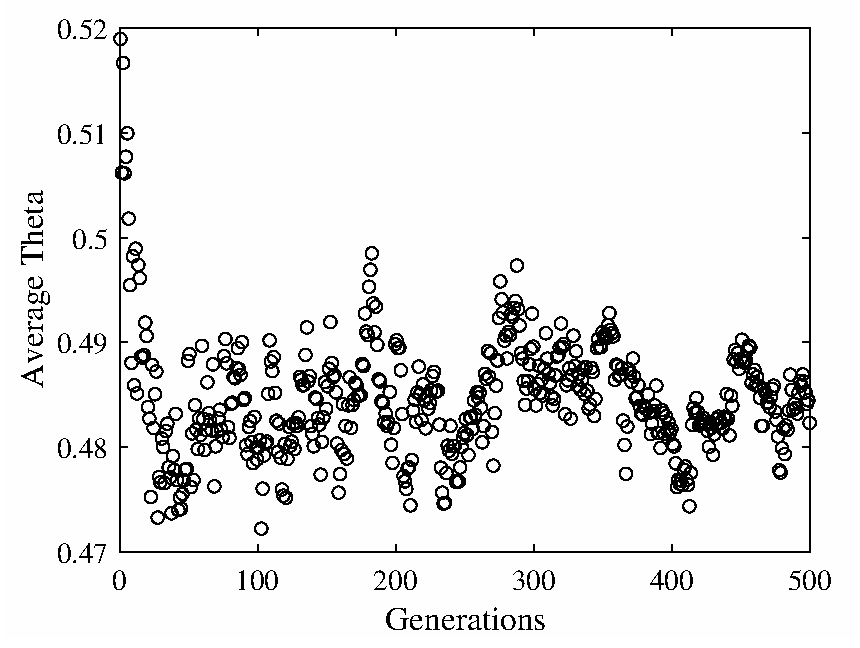
\includegraphics[width=4.0cm]{Figures/TOMs_Problem_WithBest_2_Theta.eps}} \hspace{0.5cm}
\subfloat[MEDA - Ulam\newline N-be75eec (LOP).]{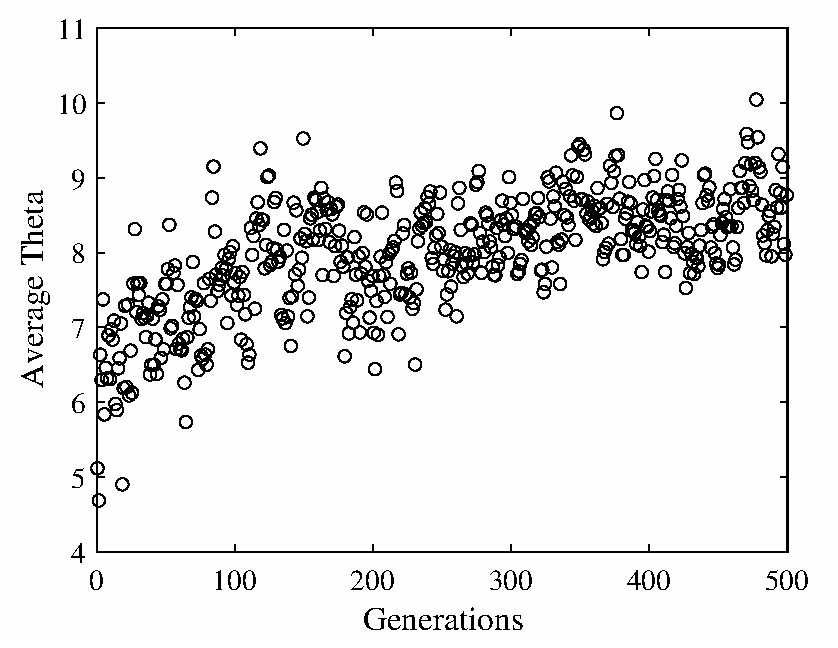
\includegraphics[width=4.0cm]
{Figures/TOMs_Problem_WithBest_1_Theta.eps}} \hspace{0.5cm}
\end{center}
\caption[caption]{Evolution of $\theta$ and average $\mathbf{\theta}$ values obtained through out the optimization (averaged across 50 repetitions).}
\label{fig:thetas}
\end{figure}

As can be seen in Fig.~\ref{fig:convergence_fitness}, in the initial phase of the optimization, the best-found solution improves rapidly. However, as the optimization progresses, the improvements become more occasional. In parallel, we can observe in Fig.~\ref{fig:thetas}, a two-phase scenario in the behavior of the $\theta$ parameter. In the first generations, it takes very low values, denoting a high spread among the solutions in the population (exploration), and later, it increases rapidly, suggesting a convergence of the population (exploitation). At this point, the probability of sampling a solution far from the consensus permutation (probably the best-found solution), is extremely low. In this sense, the practitioner of the toolbox might decide to set a lower maximum $\theta$ value in order to permit the algorithm (even with low-probability) to scape from getting stuck, or at least, to delay such scenario.

Alternatively, in order to provide some performance data regarding the toolbox, in addition to the execution times introduced in Table~\ref{tab:results}, in Fig.~\ref{fig:performance} we have introduced the average execution time required by the most relevant components of EDAs: learning, sampling and evaluation functions, which almost represent the total execution time. Results have been obtained from the execution of the EDAs carried out in the previous experiments, and by averaging computation times across the generations and repetitions.
\begin{figure}[!hbt]
\centering
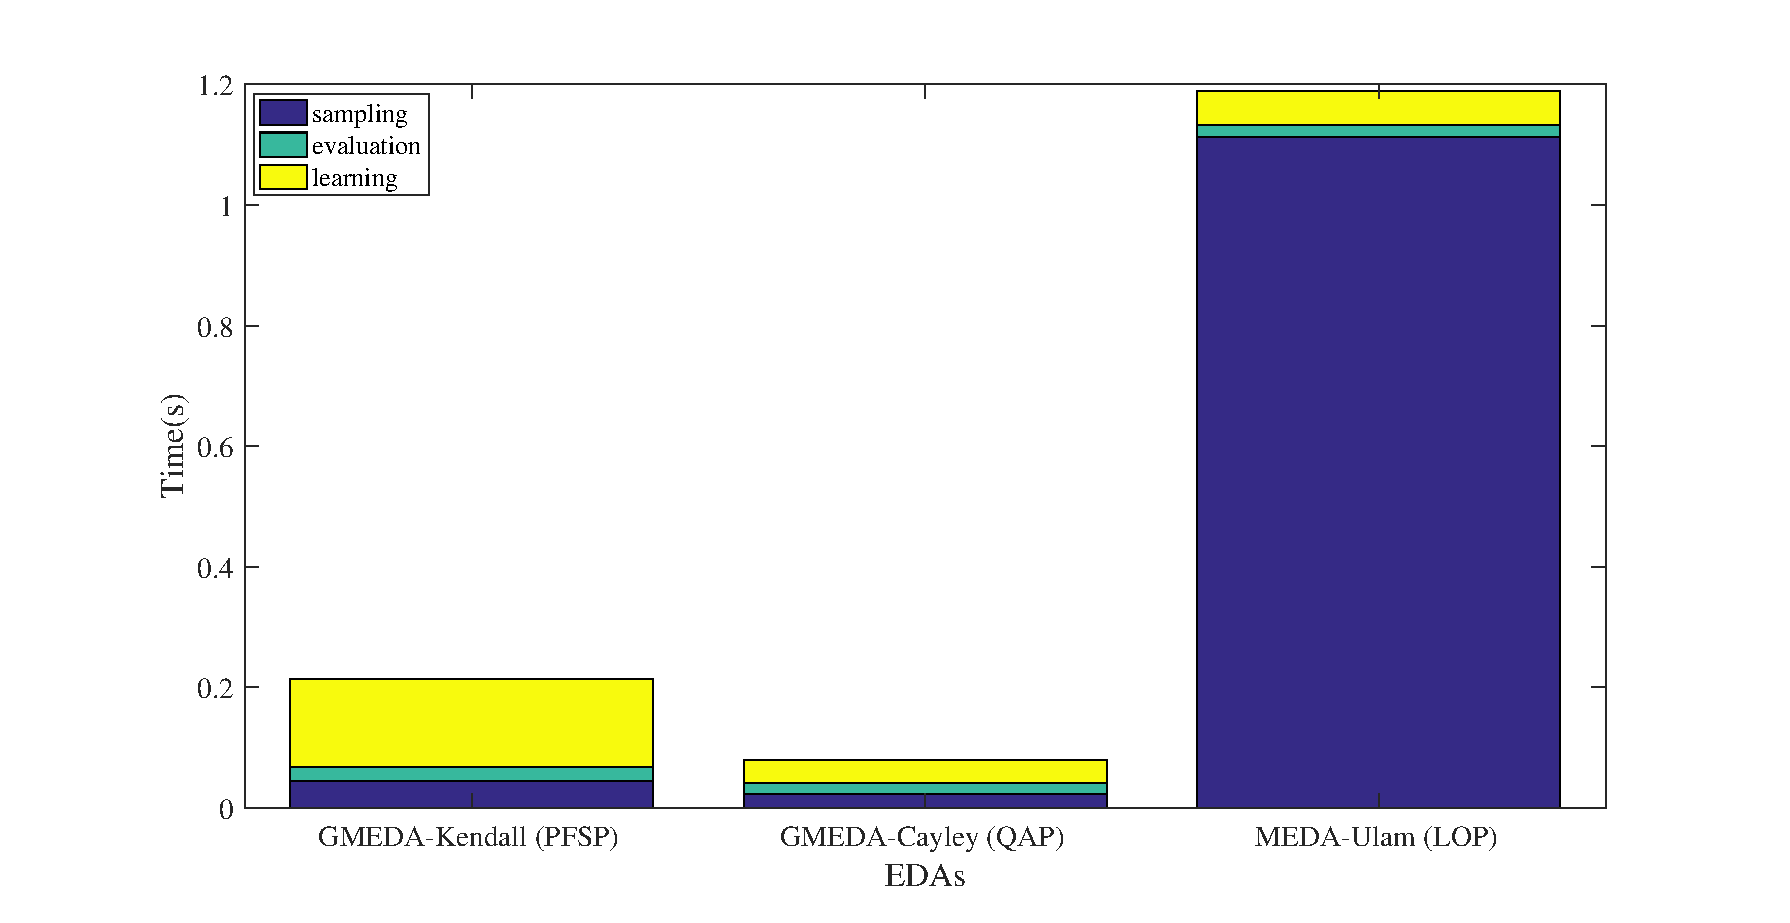
\includegraphics[width=10.0cm]{Figures/Time_EDA_Components.eps}
\caption[caption]{The average execution time required by the learning, sampling and evaluation functions.}
\label{fig:performance}
\end{figure}

The figure shows that GMEDA-Cayley is the fastest algorithm. The differences are observed in the learning and sampling steps, which are coherent with the complexity of the particular procedures reported for each distance-metric.

\section{Conclusions}\label{sec:conclusions}

Permutation-based optimization problems are present in many real-world scenarios, such as those related to logistics, planning, etc. Recently, new estimation of distribution algorithms have been proposed to solve this kind of problems in an efficient way. In this paper, we propose an extension of the Mateda 2.0 toolbox called \texttt{perm\_mateda}, designed for solving permutation-based problems. Based on two distance-based exponential probability models, the Mallows and Generalized Mallows models, the toolbox implements the functions required to run both models under the Kendall's-$\tau$, Cayley and Ulam distances. In order to provide a testbed of functions, four classical permutation problems have also been implemented: Traveling Salesman Problem, Permutation Flowshop Scheduling Problem, Linear Ordering Problem, and Quadratic Assignment Problem.  For the sake of illustrating the different functionalities, an experimental comparison of algorithms on a set of permutation problem instances has been carried out. Furthermore, in order to provide some performance data, a brief analysis of the execution times required by the learning, sampling and evaluation steps of different EDAs provided in the toolbox is introduced.

The algorithms have been implemented taking into account the modular nature of the original Mateda framework. In this sense, it will be easy for a future user to extend presented EDAs, including new probabilistic models, such as Plackett-Luce~\citep{Plackett1975,Luce1959}, add new distance metrics to existing models: for example, Hamming~\citep{Ormale1997} or even implement mixtures or kernels of the probabilistic models for permutation spaces~\cite{Santamaria2015,Ceberio2015b}. 

% Bibliography
\bibliographystyle{ACM-Reference-Format-Journals}
\bibliography{1_bibliography.bib}
                             % Sample .bib file with references that match those in
                             % the 'Specifications Document (V1.5)' as well containing
                             % 'legacy' bibs and bibs with 'alternate codings'.
                             % Gerry Murray - March 2012

% History dates
%\received{February 2007}{March 2009}{June 2009}

% Electronic Appendix
%\elecappendix
%
%\medskip
%
%\section{This is an example of Appendix section head}
%
%Channel-switching time is measured as the time length it takes for
%motes to successfully switch from one channel to another. This
%parameter impacts the maximum network throughput, because motes
%cannot receive or send any packet during this period of time, and it
%also affects the efficiency of toggle snooping in MMSN, where motes
%need to sense through channels rapidly.
%
%By repeating experiments 100 times, we get the average
%channel-switching time of Micaz motes: 24.3 $\mu$s. We then conduct
%the same experiments with different Micaz motes, as well as
%experiments with the transmitter switching from Channel 11 to other
%channels. In both scenarios, the channel-switching time does not have
%obvious changes. (In our experiments, all values are in the range of
%23.6 $\mu$s to 24.9 $\mu$s.)
%
%\section{Appendix section head}
%
%The primary consumer of energy in WSNs is idle listening. The key to
%reduce idle listening is executing low duty-cycle on nodes. Two
%primary approaches are considered in controlling duty-cycles in the
%MAC layer.
%
\end{document}
% End of v2-acmsmall-sample.tex (March 2012) - Gerry Murray, ACM


